\documentclass[10pt]{article}
\usepackage[russian]{babel}
\usepackage[utf8]{inputenc}
\usepackage{amssymb}
\usepackage{amsmath}
\usepackage{latexsym}
\usepackage{enumitem}
\usepackage[margin=2cm]{geometry}
\usepackage{tikz}
\usepackage{graphicx}
\usetikzlibrary{arrows}

\renewcommand{\leq}{\leqslant}
\renewcommand{\geq}{\geqslant}

\begin{document}

\title{Домашняя работа 5}
\author{Антон Афанасьев}
\maketitle

\begin{enumerate}
\item[6.3] Граф $k$-регулярный, значит $\delta = k$ и $\kappa(G) \leq k$. Пусть мы удалили сколько-то вершин, и граф распался на компоненты связности. Это означает, что круг, в который были расставлены наши вершины распался на несколько связных сегментов. Рассмотрим некоторый сегмент. Его крайняя правая вершина была соединена с $k/2$ вершинами справа, а раз сейчас она крайняя, то эти вершины были удалены. Его левая вершина была соединена с $k/2$ вершинами слева, но сейчас она крайняя, значит, эти вершины тоже удалены. Эти два множества вершин --- разные вершины, иначе получилось бы, что круг на них замыкается, и отрезок который мы рассматриваем --- единственный. Получили, что для того, чтобы граф распался, нужно было удалить не менее $k$ вершин.\\
Значит, $\kappa(G) = k$.

\item[6.6] Возьмем два полных графа $K_{\delta+1}$. Добавим к ним $\kappa$ вершин. Каждую из этих вершин полных подграфов, кроме одной в каждом из них, соединим с каждой из дополнительных вершин ребром. Получим граф $G_1$, у которого $\delta(G_1) = \delta$ (у вершин в полных подграфах, из которых не проводили ребра). $\kappa(G_1) = \kappa$, так как, если удалить дополнительные вершины граф распадется, а удаление меньшего количества вершин не сможет этого сделать (полные подграфы не распадутся и связь между ними тоже останется). При этом, $\lambda(G_1) = \delta$ по тем же соображениям.

Теперь добавим еще третий полный подграф $K_{\delta+1}$ и $\lambda$ вершин. Будем считать эти $\lambda$ вершин дополнительными вершинами. Каждую из дополнительных вершин соединим одним ребром с вершиной из второго полного подграфа (каждую со своей) и соединим $\delta$ ребрами с вершинами третьего полного подграфа. Получим граф $G_2$. В этом графе мы не изменили $\kappa$ и $\delta$ графа $G_1$, но теперь $\lambda(G_2) = \lambda$, так как можно удалить ребра из $\lambda$ дополнительных вершин во второй полный подграф и нарушить связность. При этом удалением меньшего числа ребер этого добиться нельзя (реберная связность $G_1$ была больше, полный подграф не распадется, а ребер из дополнительных вершин в третий подграф много).

Таким образом, мы построили граф с заданными параметрами.

\item[6.7]
\begin{enumerate}
	\item $\kappa(G) = 2,\ \lambda(G) = 4,\ \delta(G) = 4$\\
	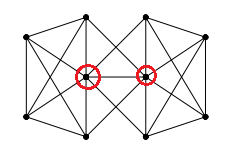
\includegraphics{graph.png}\\
	В графе нет точек сочленения, при этом, можно удалить две вершины, отмеченные на рисунке, и граф распадется. Значит, $\kappa(G) = 2$. Граф можно рассматривать, как два подграфа, соединяемые отмеченными вершинами. Удаляя 3 ребра нельзя разделить эти подграфы и нельзя нарушить связность внутри них. Но, так как есть вершина степени 4, это можно сделать удалив 4 ребра. Следовательно, $\lambda(G) = 4$.
	
	\item $\kappa(G) = 4,\ \lambda(G) = 4,\ \delta(G) = 4$\\
	Попробуем разорвать граф, удалив 3 вершины. Граф состоит из трех клик размера 4, разорвать клику удаляя 3 вершины не получится. Эти клики лежат на двух непересекающихся циклах, каждый из которых нужно разорвать в двух местах. Таким образом, удаляя только три вершины не получается сделать граф несвязным. Однако, если удалить 4 ``противоположные'' вершины, граф распадается, следовательно $\kappa(G) = 4$. Из тех же соображений реберная связность тоже равна 4 (клики лежат на двух циклах, развалить клики не получится, а каждый цикл нужно разорвать в двух местах).
\end{enumerate}

\item[6.8] У 3-регулярного графа $\delta(G) = 3$, значит, $\kappa(G) \leq 3$ и $\kappa(G) \in \{1, 2, 3\}$. Разберем эти случаи.
\begin{itemize}
	\item Пусть $\kappa(G) = 3$. Так как $\kappa(G) \leq \lambda(G) \leq \delta(G)$, $\lambda(G) = 3$.
	\item Пусть $\kappa(G) = 1$. Тогда существует вершина $v \in V(G)$, являющаяся точкой сочленения. Так как у вершины $v$ степень 3, то либо все ее ребра ведут в разные компоненты, на которые граф распадется после ее удаления, либо два ребра ведут в одну, а третье в другую (все три вести в одну не могут, иначе эта вершина не была бы точкой сочленения). Рассмотрим компоненту, в которую ведет только одно ребро из $v$. Это ребро будет являться мостом, а значит $\lambda(G) = 1$.
	\item Пусть $\kappa(G) = 2$. Тогда существует две вершины $u$ и $v$, такие, что граф распадается на компоненты связности, если их удалить. После удаления вершин $u$ и $v$ граф мог распасться не более чем на 3 компоненты связности (после удаления $u$ граф не распадется, а вершина $v$ не может соединять больше трех компонент).
	
	 И вершина $u$ и вершина $v$ должны были быть смежны с какой-либо вершиной из каждой компоненты. Если бы это было не так, например $v$ была бы не смежна ни с одной вершиной какой-то компоненты, то при удалении вершины $u$ эта компоненты оказалась бы не связанна с остальным графом, то есть вершина $u$ оказалась бы точкой сочленения. \\
	Если граф, после удаления вершин $u$ и $v$ граф распадается на три компоненты связности, то в каждую из них из $u$ и из $v$ идет по одному ребру. Значит, достаточно удалить два ребра, чтобы ``отцепить'' одну компоненту. Если граф распадается на две компоненты связности, то из $u$ в одну из этих компонент идет два ребра, а в другую одно, так же ситуация для $v$. Удалив одиночные ребра мы также развалим граф. Таким образом, в обоих случаях $\lambda(G) = 2$.
\end{itemize}
Итак, для всех возможных значений $\kappa(G)$, $\kappa(G) = \lambda(G)$.

\item[6.13] Граф $G$ --- двусвязный. Покажем, что его можно разложить на ручки, начиная с произвольного цикла. 

Начинаем с цикла. Пусть какая-то часть графа $G$ уже покрыта циклом с ручками, обозначим ее за $H$. Возьмем еще не покрытую вершину $v$ и уже покрытую вершину $u$. Так как граф двусвязный, существует цикл, проходящий через эти вершины. Некоторая часть этого цикла будет проходить еще непокрытым вершинам и ребрам. Рассмотрим отрезок пути с момента выхода из $H$ до момента захода в $H$. Если концы этого пути ($p$ и $q$) различны, то он является ручкой. Иначе, существует другой путь, начинающийся в $p$, проходящий через $v$, и возвращающийся в другую вершину из $H$. Если бы его не существовало, то точка $p$ была бы точкой сочленения. Этот другой путь будет являться ручкой.

Добавим новую ручку к $H$ и будем продолжать так до тех пор, пока мы не покроем все вершины. После этого, возможно, нужно будет еще покрыть некоторые ребра, но так как их концы лежат в $H$ они сами по себе являются ручками и их можно просто добавить.

\item[6.16] Пусть ориентированный граф является сильно-связным. Тогда, для любой пабы вершин $u,\ v$ существует путь из $v$ в $u$ и из $u$ в $v$. Следовательно, $u$ и $v$ лежат на некотором цикле. Но тогда, в соответствующем неориентированном графе эти вершины тоже лежат на цикле, а значит, их нельзя поместить в разные компоненты связности убрав только одно ребро. Никакие две вершины нельзя разделить удаляя одно ребро, следовательно неориентированный граф реберно-двусвязный.

Пусть теперь есть неориентированный, реберно-двусвязный граф. \\
Пусть он является еще и вершинно-двусвязным. Тогда его можно разбить на цикл и ручки. Ориентируем ребра на цикле в какую-нибудь сторону. Будем теперь добавлять ручки, тоже ориентируя их. Несложно заметить, что на каждом шаге получающийся граф остается сильно-связным: цикл был сильно связным, и для новой ручки, из любой вершины ручки можно попасть в любую вершину текущего графа пройдя до конца ручки в сильно-связный подграф, и при необходимости вернувшись в ручку, и так же можно из любой вершины подграфа попасть в вершины ручки, добравшись до ее начала и пройдя по ней. Значит, построенный таким образом граф будет сильно-связным.

Пусть граф не является вершинно-двусвязным. Тогда он разбивается на двусвязные компоненты. При этом, так как граф является реберно-двусвязным, компоненты двусвязности соединяются между собой только вершинами (если бы какие-то компоненты соединялись ребром, то это ребро было бы мостом). Это значит, что можно в каждой компоненте ориентировать ребра как в предыдущем случае, и такой граф будет сильно-связным.
\end{enumerate}

\end{document}
